% Options for packages loaded elsewhere
\PassOptionsToPackage{unicode}{hyperref}
\PassOptionsToPackage{hyphens}{url}
%
\documentclass[
]{article}
\usepackage{amsmath,amssymb}
\usepackage{lmodern}
\usepackage{ifxetex,ifluatex}
\ifnum 0\ifxetex 1\fi\ifluatex 1\fi=0 % if pdftex
  \usepackage[T1]{fontenc}
  \usepackage[utf8]{inputenc}
  \usepackage{textcomp} % provide euro and other symbols
\else % if luatex or xetex
  \usepackage{unicode-math}
  \defaultfontfeatures{Scale=MatchLowercase}
  \defaultfontfeatures[\rmfamily]{Ligatures=TeX,Scale=1}
\fi
% Use upquote if available, for straight quotes in verbatim environments
\IfFileExists{upquote.sty}{\usepackage{upquote}}{}
\IfFileExists{microtype.sty}{% use microtype if available
  \usepackage[]{microtype}
  \UseMicrotypeSet[protrusion]{basicmath} % disable protrusion for tt fonts
}{}
\makeatletter
\@ifundefined{KOMAClassName}{% if non-KOMA class
  \IfFileExists{parskip.sty}{%
    \usepackage{parskip}
  }{% else
    \setlength{\parindent}{0pt}
    \setlength{\parskip}{6pt plus 2pt minus 1pt}}
}{% if KOMA class
  \KOMAoptions{parskip=half}}
\makeatother
\usepackage{xcolor}
\IfFileExists{xurl.sty}{\usepackage{xurl}}{} % add URL line breaks if available
\IfFileExists{bookmark.sty}{\usepackage{bookmark}}{\usepackage{hyperref}}
\hypersetup{
  pdftitle={Modul 4},
  pdfauthor={Eva},
  hidelinks,
  pdfcreator={LaTeX via pandoc}}
\urlstyle{same} % disable monospaced font for URLs
\usepackage[margin=1in]{geometry}
\usepackage{color}
\usepackage{fancyvrb}
\newcommand{\VerbBar}{|}
\newcommand{\VERB}{\Verb[commandchars=\\\{\}]}
\DefineVerbatimEnvironment{Highlighting}{Verbatim}{commandchars=\\\{\}}
% Add ',fontsize=\small' for more characters per line
\usepackage{framed}
\definecolor{shadecolor}{RGB}{248,248,248}
\newenvironment{Shaded}{\begin{snugshade}}{\end{snugshade}}
\newcommand{\AlertTok}[1]{\textcolor[rgb]{0.94,0.16,0.16}{#1}}
\newcommand{\AnnotationTok}[1]{\textcolor[rgb]{0.56,0.35,0.01}{\textbf{\textit{#1}}}}
\newcommand{\AttributeTok}[1]{\textcolor[rgb]{0.77,0.63,0.00}{#1}}
\newcommand{\BaseNTok}[1]{\textcolor[rgb]{0.00,0.00,0.81}{#1}}
\newcommand{\BuiltInTok}[1]{#1}
\newcommand{\CharTok}[1]{\textcolor[rgb]{0.31,0.60,0.02}{#1}}
\newcommand{\CommentTok}[1]{\textcolor[rgb]{0.56,0.35,0.01}{\textit{#1}}}
\newcommand{\CommentVarTok}[1]{\textcolor[rgb]{0.56,0.35,0.01}{\textbf{\textit{#1}}}}
\newcommand{\ConstantTok}[1]{\textcolor[rgb]{0.00,0.00,0.00}{#1}}
\newcommand{\ControlFlowTok}[1]{\textcolor[rgb]{0.13,0.29,0.53}{\textbf{#1}}}
\newcommand{\DataTypeTok}[1]{\textcolor[rgb]{0.13,0.29,0.53}{#1}}
\newcommand{\DecValTok}[1]{\textcolor[rgb]{0.00,0.00,0.81}{#1}}
\newcommand{\DocumentationTok}[1]{\textcolor[rgb]{0.56,0.35,0.01}{\textbf{\textit{#1}}}}
\newcommand{\ErrorTok}[1]{\textcolor[rgb]{0.64,0.00,0.00}{\textbf{#1}}}
\newcommand{\ExtensionTok}[1]{#1}
\newcommand{\FloatTok}[1]{\textcolor[rgb]{0.00,0.00,0.81}{#1}}
\newcommand{\FunctionTok}[1]{\textcolor[rgb]{0.00,0.00,0.00}{#1}}
\newcommand{\ImportTok}[1]{#1}
\newcommand{\InformationTok}[1]{\textcolor[rgb]{0.56,0.35,0.01}{\textbf{\textit{#1}}}}
\newcommand{\KeywordTok}[1]{\textcolor[rgb]{0.13,0.29,0.53}{\textbf{#1}}}
\newcommand{\NormalTok}[1]{#1}
\newcommand{\OperatorTok}[1]{\textcolor[rgb]{0.81,0.36,0.00}{\textbf{#1}}}
\newcommand{\OtherTok}[1]{\textcolor[rgb]{0.56,0.35,0.01}{#1}}
\newcommand{\PreprocessorTok}[1]{\textcolor[rgb]{0.56,0.35,0.01}{\textit{#1}}}
\newcommand{\RegionMarkerTok}[1]{#1}
\newcommand{\SpecialCharTok}[1]{\textcolor[rgb]{0.00,0.00,0.00}{#1}}
\newcommand{\SpecialStringTok}[1]{\textcolor[rgb]{0.31,0.60,0.02}{#1}}
\newcommand{\StringTok}[1]{\textcolor[rgb]{0.31,0.60,0.02}{#1}}
\newcommand{\VariableTok}[1]{\textcolor[rgb]{0.00,0.00,0.00}{#1}}
\newcommand{\VerbatimStringTok}[1]{\textcolor[rgb]{0.31,0.60,0.02}{#1}}
\newcommand{\WarningTok}[1]{\textcolor[rgb]{0.56,0.35,0.01}{\textbf{\textit{#1}}}}
\usepackage{graphicx}
\makeatletter
\def\maxwidth{\ifdim\Gin@nat@width>\linewidth\linewidth\else\Gin@nat@width\fi}
\def\maxheight{\ifdim\Gin@nat@height>\textheight\textheight\else\Gin@nat@height\fi}
\makeatother
% Scale images if necessary, so that they will not overflow the page
% margins by default, and it is still possible to overwrite the defaults
% using explicit options in \includegraphics[width, height, ...]{}
\setkeys{Gin}{width=\maxwidth,height=\maxheight,keepaspectratio}
% Set default figure placement to htbp
\makeatletter
\def\fps@figure{htbp}
\makeatother
\setlength{\emergencystretch}{3em} % prevent overfull lines
\providecommand{\tightlist}{%
  \setlength{\itemsep}{0pt}\setlength{\parskip}{0pt}}
\setcounter{secnumdepth}{-\maxdimen} % remove section numbering
\ifluatex
  \usepackage{selnolig}  % disable illegal ligatures
\fi

\title{Modul 4}
\author{Eva}
\date{9/30/2021}

\begin{document}
\maketitle

\begin{enumerate}
\def\labelenumi{\arabic{enumi}.}
\tightlist
\item
  Gunakan operator aksesor (\$) untuk mengakses variabel populasi dan
  menyimpannya pada objek baru ``pop''. Kemudian gunakan fungsi sort
  untuk mengurutkan variabel ``pop''. Pada langkah terakhir, gunakan
  operator ({[}) untuk menampilkan nilai populasi terkecil
\end{enumerate}

\begin{Shaded}
\begin{Highlighting}[]
\NormalTok{pop }\OtherTok{=}\NormalTok{ murders}\SpecialCharTok{$}\NormalTok{population}
\NormalTok{pop }\OtherTok{=} \FunctionTok{sort}\NormalTok{(pop)}
\NormalTok{pop[}\DecValTok{1}\NormalTok{]}
\end{Highlighting}
\end{Shaded}

\begin{verbatim}
## [1] 563626
\end{verbatim}

\begin{enumerate}
\def\labelenumi{\arabic{enumi}.}
\setcounter{enumi}{1}
\tightlist
\item
  Tampilkan indeks dari data yang memiliki nilai populasi terkecil.
  Petunjuk: gunakan fungsi order
\end{enumerate}

\begin{Shaded}
\begin{Highlighting}[]
\NormalTok{index }\OtherTok{=} \FunctionTok{order}\NormalTok{(murders}\SpecialCharTok{$}\NormalTok{population)}
\NormalTok{index[}\DecValTok{1}\NormalTok{]}
\end{Highlighting}
\end{Shaded}

\begin{verbatim}
## [1] 51
\end{verbatim}

\begin{enumerate}
\def\labelenumi{\arabic{enumi}.}
\setcounter{enumi}{2}
\tightlist
\item
  Dengan fungsi which.min, Tulis satu baris kode yang dapat menampilkan
  hasil yang sama dengan langkah diatas.
\end{enumerate}

\begin{Shaded}
\begin{Highlighting}[]
\FunctionTok{which.min}\NormalTok{(murders}\SpecialCharTok{$}\NormalTok{population)}
\end{Highlighting}
\end{Shaded}

\begin{verbatim}
## [1] 51
\end{verbatim}

\begin{enumerate}
\def\labelenumi{\arabic{enumi}.}
\setcounter{enumi}{3}
\tightlist
\item
  Tampilkan nama negara yang memiliki populasi terkecil
\end{enumerate}

\begin{Shaded}
\begin{Highlighting}[]
\NormalTok{i\_min }\OtherTok{=} \FunctionTok{which.min}\NormalTok{(murders}\SpecialCharTok{$}\NormalTok{population)}
\NormalTok{murders}\SpecialCharTok{$}\NormalTok{state[i\_min]}
\end{Highlighting}
\end{Shaded}

\begin{verbatim}
## [1] "Wyoming"
\end{verbatim}

\begin{enumerate}
\def\labelenumi{\arabic{enumi}.}
\setcounter{enumi}{4}
\tightlist
\item
  Untuk membuat data frame baru, contoh script yang dapat digunakan
  adalah sebagai berikut:
\end{enumerate}

\begin{Shaded}
\begin{Highlighting}[]
\NormalTok{temp }\OtherTok{\textless{}{-}} \FunctionTok{c}\NormalTok{(}\DecValTok{35}\NormalTok{, }\DecValTok{88}\NormalTok{, }\DecValTok{42}\NormalTok{, }\DecValTok{84}\NormalTok{, }\DecValTok{81}\NormalTok{, }\DecValTok{30}\NormalTok{)}
\NormalTok{city }\OtherTok{\textless{}{-}} \FunctionTok{c}\NormalTok{(}\StringTok{"Beijing"}\NormalTok{, }\StringTok{"Lagos"}\NormalTok{, }\StringTok{"Paris"}\NormalTok{, }\StringTok{"Rio de Janeiro"}\NormalTok{, }\StringTok{"San Juan"}\NormalTok{, }\StringTok{"Toronto"}\NormalTok{)}
\NormalTok{city\_temps }\OtherTok{\textless{}{-}} \FunctionTok{data.frame}\NormalTok{(}\AttributeTok{name =}\NormalTok{ city, }\AttributeTok{temperature =}\NormalTok{ temp)}
\end{Highlighting}
\end{Shaded}

Gunakan fungsi rank untuk menentukan peringkat populasi dari tiap negara
bagian, dimulai dari nilai terkecil hingga terbesar. Simpan hasil
pemeringkatan di objek baru ``ranks'', lalu buat data frame baru yang
berisi nama negara bagian dan peringkatnya dengan nama ``my\_df''.

\begin{Shaded}
\begin{Highlighting}[]
\NormalTok{temp }\OtherTok{=}\NormalTok{ murders}\SpecialCharTok{$}\NormalTok{state}
\NormalTok{ranks }\OtherTok{=} \FunctionTok{rank}\NormalTok{(murders}\SpecialCharTok{$}\NormalTok{population)}
\NormalTok{my\_df }\OtherTok{\textless{}{-}} \FunctionTok{data.frame}\NormalTok{(}\AttributeTok{name=}\NormalTok{temp, ranks)}
\NormalTok{my\_df}
\end{Highlighting}
\end{Shaded}

\begin{verbatim}
##                    name ranks
## 1               Alabama    29
## 2                Alaska     5
## 3               Arizona    36
## 4              Arkansas    20
## 5            California    51
## 6              Colorado    30
## 7           Connecticut    23
## 8              Delaware     7
## 9  District of Columbia     2
## 10              Florida    49
## 11              Georgia    44
## 12               Hawaii    12
## 13                Idaho    13
## 14             Illinois    47
## 15              Indiana    37
## 16                 Iowa    22
## 17               Kansas    19
## 18             Kentucky    26
## 19            Louisiana    27
## 20                Maine    11
## 21             Maryland    33
## 22        Massachusetts    38
## 23             Michigan    43
## 24            Minnesota    31
## 25          Mississippi    21
## 26             Missouri    34
## 27              Montana     8
## 28             Nebraska    14
## 29               Nevada    17
## 30        New Hampshire    10
## 31           New Jersey    41
## 32           New Mexico    16
## 33             New York    48
## 34       North Carolina    42
## 35         North Dakota     4
## 36                 Ohio    45
## 37             Oklahoma    24
## 38               Oregon    25
## 39         Pennsylvania    46
## 40         Rhode Island     9
## 41       South Carolina    28
## 42         South Dakota     6
## 43            Tennessee    35
## 44                Texas    50
## 45                 Utah    18
## 46              Vermont     3
## 47             Virginia    40
## 48           Washington    39
## 49        West Virginia    15
## 50            Wisconsin    32
## 51              Wyoming     1
\end{verbatim}

\begin{enumerate}
\def\labelenumi{\arabic{enumi}.}
\setcounter{enumi}{5}
\tightlist
\item
  Ulangi langkah sebelumnya, namun kali ini urutkan my\_df dengan fungsi
  order agar data yang ditampilkan merupakan data yang telah diurutkan
  dari populasi yang paling tidak padat hingga ke yang terpadat.
  Petunjuk: buat objek ``ind'' yang akan menyimpan indeks yang
  diperlukan dalam mengurutkan data populasi
\end{enumerate}

\begin{Shaded}
\begin{Highlighting}[]
\NormalTok{ranks }\OtherTok{\textless{}{-}} \FunctionTok{rank}\NormalTok{(murders}\SpecialCharTok{$}\NormalTok{population)}
\NormalTok{my\_df }\OtherTok{\textless{}{-}} \FunctionTok{data.frame}\NormalTok{(}\AttributeTok{state =}\NormalTok{ murders}\SpecialCharTok{$}\NormalTok{state, }
\AttributeTok{ranks =}\NormalTok{ ranks)}
\NormalTok{ind }\OtherTok{\textless{}{-}} \FunctionTok{order}\NormalTok{(my\_df}\SpecialCharTok{$}\NormalTok{ranks)}
\NormalTok{my\_df }\OtherTok{\textless{}{-}} \FunctionTok{data.frame}\NormalTok{(}\AttributeTok{state =}\NormalTok{ murders}\SpecialCharTok{$}\NormalTok{state[ind], }
\AttributeTok{ranks =} \DecValTok{1}\SpecialCharTok{:}\FunctionTok{nrow}\NormalTok{(my\_df))}
\NormalTok{my\_df}
\end{Highlighting}
\end{Shaded}

\begin{verbatim}
##                   state ranks
## 1               Wyoming     1
## 2  District of Columbia     2
## 3               Vermont     3
## 4          North Dakota     4
## 5                Alaska     5
## 6          South Dakota     6
## 7              Delaware     7
## 8               Montana     8
## 9          Rhode Island     9
## 10        New Hampshire    10
## 11                Maine    11
## 12               Hawaii    12
## 13                Idaho    13
## 14             Nebraska    14
## 15        West Virginia    15
## 16           New Mexico    16
## 17               Nevada    17
## 18                 Utah    18
## 19               Kansas    19
## 20             Arkansas    20
## 21          Mississippi    21
## 22                 Iowa    22
## 23          Connecticut    23
## 24             Oklahoma    24
## 25               Oregon    25
## 26             Kentucky    26
## 27            Louisiana    27
## 28       South Carolina    28
## 29              Alabama    29
## 30             Colorado    30
## 31            Minnesota    31
## 32            Wisconsin    32
## 33             Maryland    33
## 34             Missouri    34
## 35            Tennessee    35
## 36              Arizona    36
## 37              Indiana    37
## 38        Massachusetts    38
## 39           Washington    39
## 40             Virginia    40
## 41           New Jersey    41
## 42       North Carolina    42
## 43             Michigan    43
## 44              Georgia    44
## 45                 Ohio    45
## 46         Pennsylvania    46
## 47             Illinois    47
## 48             New York    48
## 49              Florida    49
## 50                Texas    50
## 51           California    51
\end{verbatim}

\begin{enumerate}
\def\labelenumi{\arabic{enumi}.}
\setcounter{enumi}{6}
\tightlist
\item
  Untuk keperluan analisis data, akan dibuat plot yang memvisualisasikan
  total pembunuhan terhadap populasi dan mengidentifikasi hubungan
  antara keduanya. Script yang digunakan:
\end{enumerate}

\begin{Shaded}
\begin{Highlighting}[]
\NormalTok{population\_in\_millions }\OtherTok{\textless{}{-}}\NormalTok{ murders}\SpecialCharTok{$}\NormalTok{population}\SpecialCharTok{/}\DecValTok{10}\SpecialCharTok{\^{}}\DecValTok{6}
\NormalTok{total\_gun\_murders }\OtherTok{\textless{}{-}}\NormalTok{ murders}\SpecialCharTok{$}\NormalTok{total}
\FunctionTok{plot}\NormalTok{(population\_in\_millions,total\_gun\_murders)}
\end{Highlighting}
\end{Shaded}

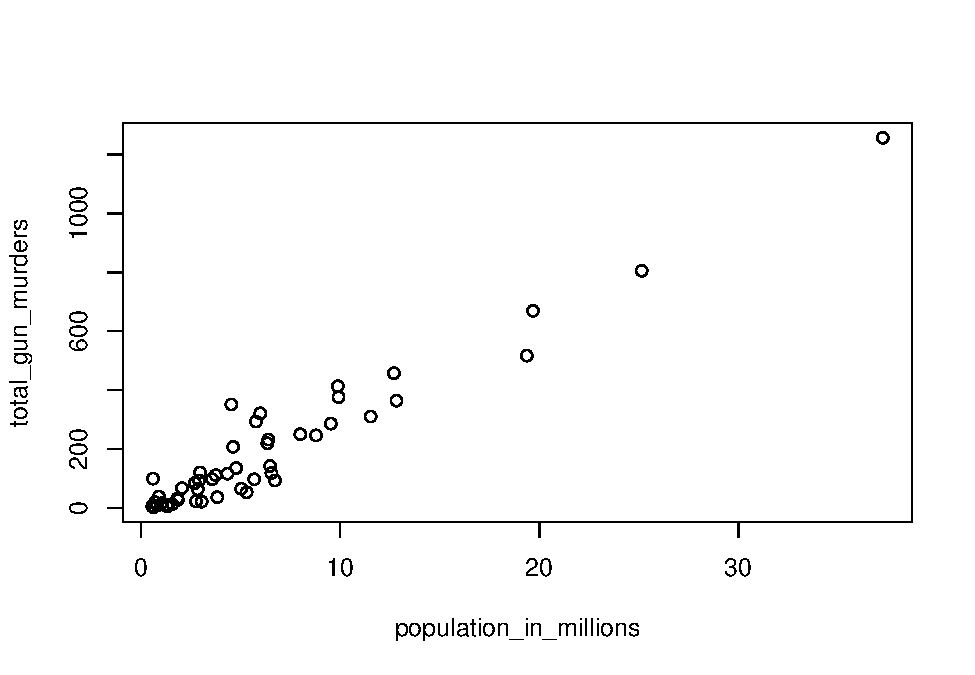
\includegraphics{Latihan3_123190027_files/figure-latex/unnamed-chunk-8-1.pdf}
Perlu diingat bahwa beberapa negara bagian memiliki populasi di bawah 5
juta, sehingga untuk mempermudah analisis, buat plot dalam skala log.
Transformasi nilai variabel menggunakan transformasi log10,kemudian
tampilkan plot-nya.

\begin{Shaded}
\begin{Highlighting}[]
\NormalTok{population\_in\_log10 }\OtherTok{\textless{}{-}} \FunctionTok{log10}\NormalTok{(population\_in\_millions)}
\NormalTok{total\_gun\_murders\_log10 }\OtherTok{\textless{}{-}} \FunctionTok{log10}\NormalTok{(total\_gun\_murders)}
\FunctionTok{plot}\NormalTok{(population\_in\_log10,total\_gun\_murders\_log10)}
\end{Highlighting}
\end{Shaded}

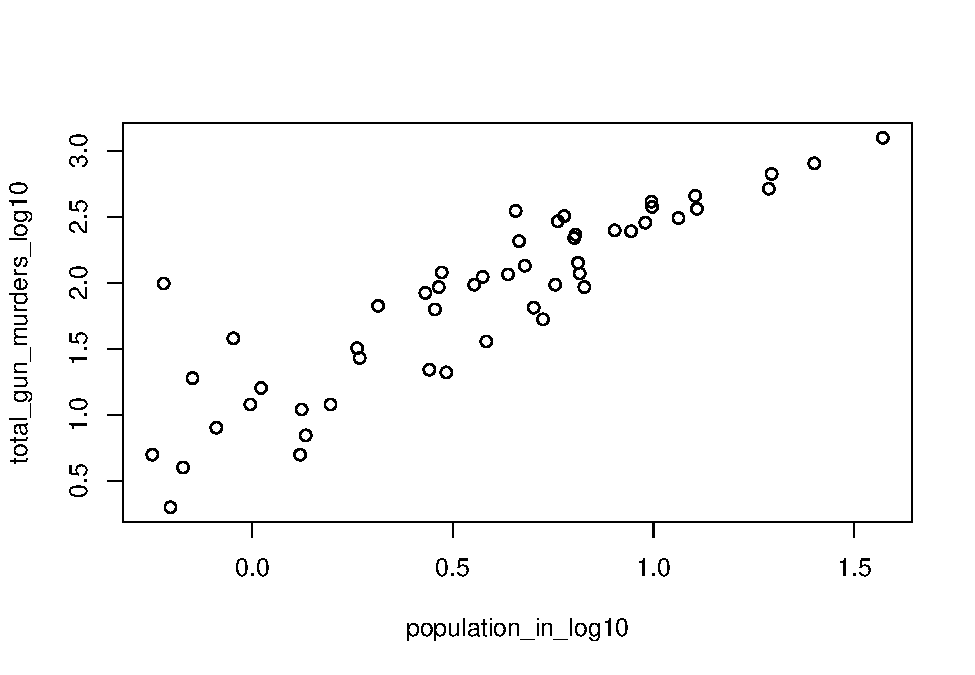
\includegraphics{Latihan3_123190027_files/figure-latex/unnamed-chunk-9-1.pdf}
8. Buat histogram dari populasi negara bagian.

\begin{Shaded}
\begin{Highlighting}[]
\NormalTok{Population }\OtherTok{=}\NormalTok{ murders}\SpecialCharTok{$}\NormalTok{population}\SpecialCharTok{/}\DecValTok{10}\SpecialCharTok{\^{}}\DecValTok{6}
\FunctionTok{hist}\NormalTok{(Population)}
\end{Highlighting}
\end{Shaded}

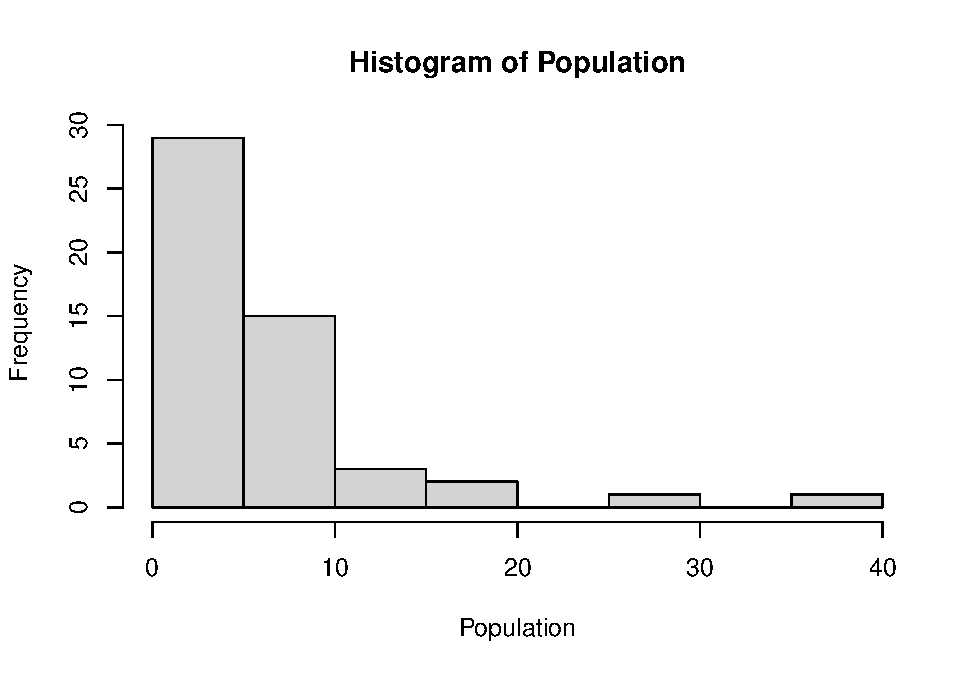
\includegraphics{Latihan3_123190027_files/figure-latex/unnamed-chunk-10-1.pdf}
9. Hasilkan boxplot dari populasi negara bagian berdasarkan wilayahnya

\begin{Shaded}
\begin{Highlighting}[]
\NormalTok{murders}\SpecialCharTok{$}\NormalTok{rate }\OtherTok{\textless{}{-}} \FunctionTok{with}\NormalTok{(murders, murders}\SpecialCharTok{$}\NormalTok{population}\SpecialCharTok{/}\DecValTok{10}\SpecialCharTok{\^{}}\DecValTok{6}\NormalTok{)}
\FunctionTok{boxplot}\NormalTok{(rate}\SpecialCharTok{\textasciitilde{}}\NormalTok{region, }\AttributeTok{data =}\NormalTok{ murders)}
\end{Highlighting}
\end{Shaded}

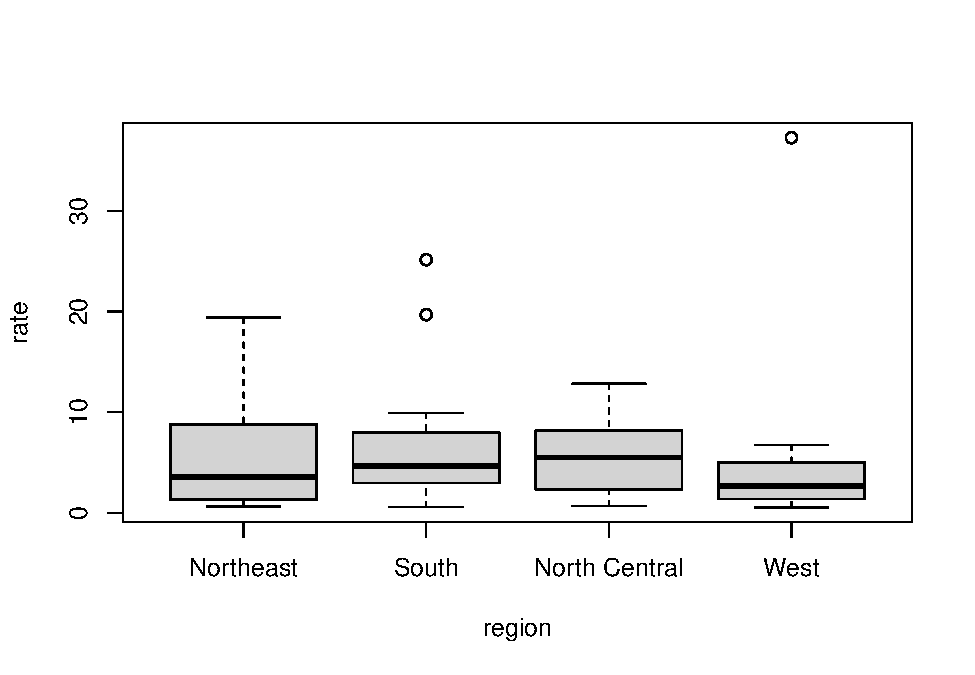
\includegraphics{Latihan3_123190027_files/figure-latex/unnamed-chunk-11-1.pdf}

\end{document}
